\documentclass{article}
\usepackage{pgfplots}
\usepackage{listings}
\usepackage{amsfonts}
\usepackage{fancybox, calc}
\lstset{language=Matlab, breaklines=true, basicstyle=\footnotesize}
\lstset{numbers=left, numberstyle=\tiny, stepnumber=1, numbersep=-6pt}
\setlength{\parskip}{\baselineskip}
\renewcommand{\baselinestretch}{1}
\usepackage{amssymb,amsmath}
\usepackage[spanish]{babel}
\usepackage[utf8]{inputenc}
\usepackage[left=4cm,right=3cm,top=4cm,bottom=3cm]{geometry}
\usepackage{graphicx}
\graphicspath{control/}
\setlength{\parskip}{\baselineskip}
\title{INSTITUTO TECNOLÓGICO DE MORELIA\\ **Análisis de un sistema de primer orden**}
\author{Alumnos: Enesto Prado Rodríguez (14120085)\\Juan Pablo Leon Pascual (15122003) \\ \\ Profesor: Gerardo Marx Chávez Campos \\ \\ Materia: Control 1}

\begin{document}
\maketitle
\newpage\section{INTRODUCCIÓN}
El control en si, ha sido muy importante en estos tiempos ya que procesos de diseño y fabricación ha facilitado hoy en día  gran porcentaje el control automotriz, sistemas roboticos, analógicos, etc. Todo lo anterior se realiza básicamente con la ayuda de la transformada de laplace, entendimiento de problemas mecánicos que se pueden hacer analogías con sistemas electrónicos, esto se podría hacer para facilitar la resolución y todo esto nos lleva a una representación del problema de ecuaciones diferenciales.

 La representación matemática de sistemas lineales, la cual presenta las
 diversas formas de representación de sistemas lineales desde el punto de vista matemático y gráfico, útiles
 para las diversas técnicas existentes en el control de procesos.

Trabajar en el dominio de Laplace no solamente es útil para la resolución matemática de ecuaciones sino que se presta especialmente para ser utilizado con el concepto de
función de transferencia. En general un proceso recibe una entrada u(t) y genera una
salida y(t). Si llevamos estas señales al dominio de Laplace tendremos una entrada
U(s) que genera una salida Y(s). La función que relaciona salida con entrada se
denomina función de transferencia g(s). \\
De modo que Y(s) = g(s)*U(s) .

Un sistema de primer orden está caracterizados principalmente por tener solamente un elemento capaz de almacenar energía y por lo anterior estarán estos sistemas representados por ecuaciones de primer orden.

Hay cuatro tipos de representar sistemas de primer orden que pueden ser:\\
Eléctrico.\\
Mecánico.\\
Hidráulico.\\
Térmicos.\\



\newpage\section{METODOLOGÍA}
Partimos del diagrama llenado de un tinaco y su salida. Al analizar tal diagrama procedemos a analizar sus variantes, para obtener la función de transferencia.

\begin{figure}[h!]
	\centering
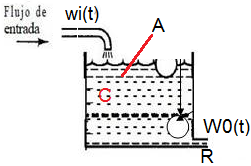
\includegraphics{C:/Users/ERNESTO/Pictures/control/a1.png}
\caption{Diagrama del problema a resolver}
\end{figure}

Entonces nos basamos en el comportamiento general del sistema de primer orden, el cual se basa en la siguiente ecuación diferencial de primer orden:
\begin{equation}
f =\sum_{}^{}E_{in} + \sum_{}^{}E_{gen} +\sum_{}^{}E_{Acc}
\end{equation}

\begin{equation}
wi(t)= \frac{Adh(t)}{dt} + wo(t)
\end{equation}

\begin{equation}
wi(t)= \frac{Rsh(t)}{R} + C \frac{dh(t)}{dt}
\end{equation}

\begin{equation}
wi(t)= Re - Ce \frac{dh(t)}{dt}
\end{equation}
\begin{figure}[h!]
	\centering
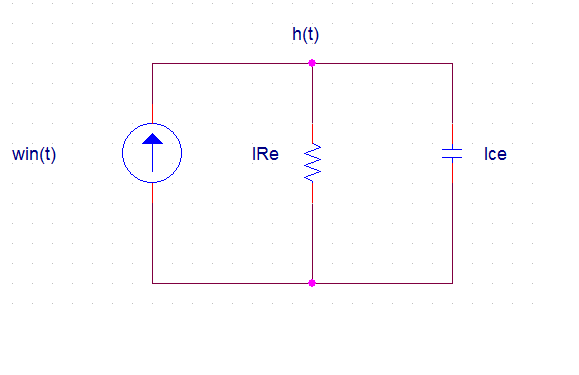
\includegraphics{../../Pictures/control/circuito1}
	\caption{Circuito}
\end{figure}\\
Ecuaciones del circuito
\begin{equation}
I_{Re} = \frac{h(t)}{Re}
\end{equation}

\begin{equation}
Re = \frac{R}{ry}
\end{equation}

Enseguida realizamos el analisis con un circuito para facilitar la resolución y aplicamos la transformada de laplace.

Transformada

\begin{equation}
win(s)= \frac{h(s)}{Re} + CeSh(s)+h(0)
\end{equation}

\begin{equation}
\frac{win(s)}{h(s)}=[Ce(s)+\frac{1}{Re}] [\frac{\frac{1}{Ce}} { \frac{1}{Ce}}]
\end{equation}


\begin{equation}
\frac{win(s)}{h(s)}=[\frac{Ce(s)Re+1}{Re}] [\frac{\frac{1}{Ce}} { \frac{1}{Ce}}]
\end{equation}

\begin{equation}
h(s)=[\frac{h(s)}{win(s)} + [\frac{Re} {1+ReCeS}]
\end{equation}
FRACCIONES PARCIALES
%%%%%%%%%%%%%%%%%%%%%%%%%%%%%%%%%%%%%% FRACCIONES PARCIALES

\begin{equation}
\frac{h(s)}{X(s)}=\frac{bs+c}{s+a}
\end{equation}

\begin{equation}
h(s)=\frac{1}{s}[\frac{bs+c}{s+a}]
\end{equation}

\begin{equation}
\frac{bs+c}{s(s+a)}]=\frac{A}{s}+\frac{b}{s+a}
\end{equation}

\begin{equation}
bs+c=A(s+a)+Bs
\end{equation}

\begin{equation}
bs+c=As+Aa+Bs
\end{equation}
tomamos solo las variables que no tienen "s" y despejamos "A"
\begin{equation}
c=Aa
\end{equation}

\begin{equation}
A=\frac{c}{a}
\end{equation}
de la ecuacion
\begin{equation}
bs+c=As+Aa+Bs
\end{equation}
tomamos las que tienen "s", despejamos "B" y sustituimos el valor de "A" para obtener el valor de "B"
\begin{equation}
bs=As+Bs
\end{equation}

\begin{equation}
B=b-\frac{c}{a}
\end{equation}
Entonces nos queda 
\begin{equation}
y(t)=\frac{c}{as}+\frac{b-\frac{c}{a}}{s+a}
\end{equation}

transformada inversa de laplace
\begin{equation}
y(t)=\frac{c}{a}+(b-\frac{c}{a})e^{-at}
\end{equation}

\begin{figure}[h!]
	\centering
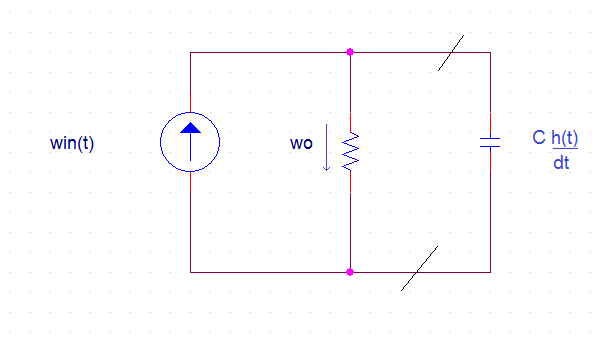
\includegraphics{../../Pictures/control/circuito2}
	\caption{wi(t) mayor w0(t)}.\\
	Cuando wi(t) = wo(t) hacemos la analogía del circuito como si el capacitor estuviera cortocircuitado.
\end{figure}\\
\begin{equation}
win(t)=wo(t)
\end{equation}
reprecentamos la cantidad de agua de entrada

\begin{equation}
Y(s)=a
\end{equation}

\section{RESULTADOS Y DISCUSIÓN:}
Para la realización o programación de nuestro código tomamos como base el código proporcionado por el profesor, tal código no lo modificamos tanto, ya que solo era necesario introducirle primero que nada el valor de las variables y por su puesto la transformada inversa de laplace o la función del tiempo. 
\begin{lstlisting}[frame=single]
      // Copyright (C) 2017 - Instituto Tecnológico de Morelia 
      // by Gerardo Marx Chavez-Campos
      // This code has been developed for educational propouses
      // the institution and author do not guarantee  the proper
      // functionality of the code.
      // Date of creation: Oct 2, 2017
      s = %s // The quicker alternative to using s =
      poly (0 , 's' ) 
      // Gain and time constant
      K = 1;  
      Tau = 1; 
      simpleSys=syslin('c', K/(1+Tau*s))
      t=0:0.01:15;
      y=csim('step', t, simpleSys)
      plot(t,y)

\end{lstlisting}
Este es el código proporcionado por el profesor donde utiliza valor de taou. y el resultado que arroja es muy similar o igual al resultado del código que realizamos nosotros.\\
\begin{figure}[h!]
	\centering
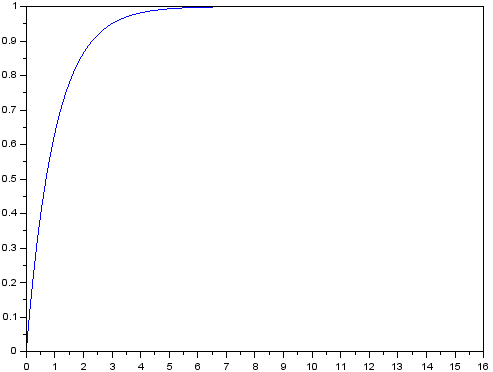
\includegraphics{../../Pictures/control/a7}
	\caption{wi(t) mayor w0(t)}
\end{figure}\\
\begin{lstlisting}[frame=single]
     //Entrada mayor que la salida wi(t))>w0(t))
     s = %s // The quicker alternative to using s
     a=1;  
     b=0;
     c=1;
     t=0:0.01:15;
     h=(c/a)+(b-c/a)*(exp(-a*t))//funcion del tiempo que se obtuvo del analisis del problema
     plot(t,h)//graficar el taou vs la funcion
\end{lstlisting}
Este código nos arrojara un resultado de cuando la entrada wi(t) es mayor a la salida wo(t), para esto es necesario darle los valores correctos a, b y c.\\
\begin{figure}[h!]
		\centering
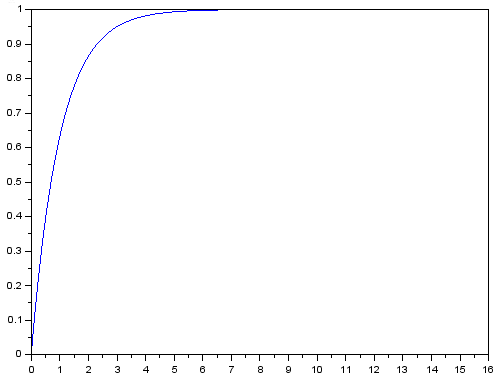
\includegraphics{C:/Users/ERNESTO/Pictures/control/a2.png}
		\caption{wi(t) mayor w0(t)}
			\label{fig:C:/Users/ERNESTO/Pictures/control/a2.png}
	\end{figure}\\
En la figura \ref{fig:C:/Users/ERNESTO/Pictures/control/a2.png} podemos apreciar el comportamiento de cuando la entra es mayor que la salida y lo podemos hacer la analogía cuando un tinaco se llena ya que en este caso la cantidad de agua que se le introduce al tinaco es mayor que la cantidad de agua que sale y por lo tanto el tinaco tendrá una apariencia de que su nivel de agua no baja a pesar de que tiene una salida.\\
\begin{lstlisting}[frame=single]
       //Entrada igual que la salida wi(t) = w0(t)
       s = %s // The quicker alternative to using s
       a=1;  
       b=7;
       c=7;
       t=0:0.01:15;
       h=(c/a)+(b-c/a)*(exp(-a*t))//funcion del tiempo que se obtuvo del analisis del problema
       plot(t,h)//graficar el taou vs la funcion
\end{lstlisting}

Este código nos arrojara un resultado de cuando la entrada wi(t) es igual a la salida wo(t), para esto es necesario darle los valores correctos a, b y c. Lo que nosotros notamos para que la entrada sea igual a la salida es necesario darle valores a menores que b y c, tales valores (b y c) fue necesario darles un valor igual.\\
\begin{figure}[h!]
	\centering
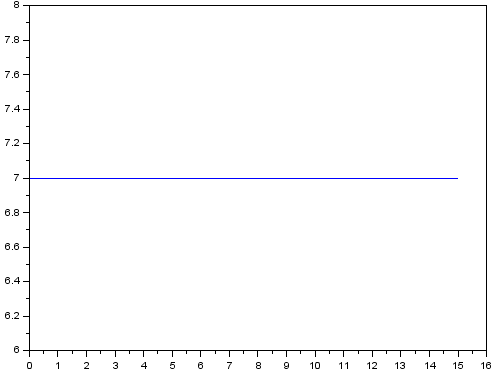
\includegraphics{C:/Users/ERNESTO/Pictures/control/a3.png}
	\caption{Grafica wi(t) = w0(t)}
	\label{fig:C:/Users/ERNESTO/Pictures/control/a3.png}
\end{figure}\\
En la figura \ref{fig:C:/Users/ERNESTO/Pictures/control/a3.png} podemos apreciar el comportamiento de cuando la entra es igual que la salida y lo podemos hacer la analogía cuando un tinaco se llena ya que en este caso la cantidad de agua que se le introduce al tinaco es igual que la cantidad de agua que sale y por lo tanto el tinaco tendrá el mismo nivel de agua.\\
\begin{lstlisting}[frame=single]
      //Entrada menor que la salida wi(t)< w0(t)
      s = %s // The quicker alternative to using s
      a=2;  
      b=3;
      c=2;
      t=0:0.01:15;
      h=(c/a)+(b-c/a)*(exp(-a*t))//funcion del tiempo que se obtuvo del analisis del problema
      plot(t,h)//graficar el taou vs la funcion

\end{lstlisting}
Este código nos arrojara un resultado de cuando la entrada wi(t) es menor a la salida wo(t), para esto es necesario darle los valores correctos a, b y c.\\
\begin{figure}[h!]
	\centering
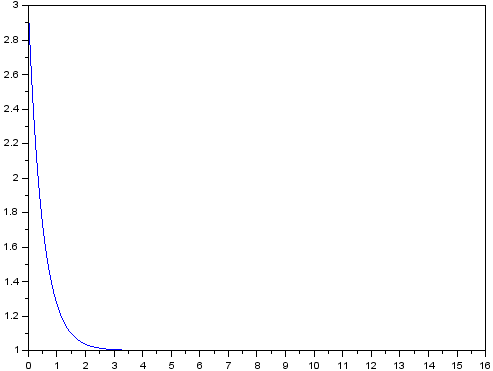
\includegraphics{C:/Users/ERNESTO/Pictures/control/a4.png}
	\caption{Gráfica wi(t) menor w0(t)}
	\label{fig:C:/Users/ERNESTO/Pictures/control/a4.png}
\end{figure}\\
En la figura \ref{fig:C:/Users/ERNESTO/Pictures/control/a4.png} podemos apreciar el comportamiento de cuando la entra es menor que la salida y lo podemos hacer la analogía cuando un tinaco se llena ya que en este caso la cantidad de agua que se le introduce al tinaco es menor que la cantidad de agua que sale y por lo tanto el tinaco tendrá una apariencia de que su nivel de agua nunca se llenara.

\begin{lstlisting}[frame=single]
     //Entrada mayor que la salida wi(t)> w0(t)
     s = %s // The quicker alternative to using s
     a=1;  
     b=0;
     c=1;
     t=0:0.01:15;
     h=(c/a)+(b-c/a)*(exp(-a*t))//funcion del tiempo que se obtuvo del analisis del problema
     plot(t,h)//graficar el taou vs la funcion
 
     //Entrada igual que la salida wi(t)= w0(t)
     s = %s // The quicker alternative to using s
     a=1;  
     b=2;
     c=2;
     t=0:0.01:15;
     h=(c/a)+(b-c/a)*(exp(-a*t))//funcion del tiempo que se obtuvo del analisis del problema
     plot(t,h)//graficar el taou vs la funcion

     //Entrada menor que la salida wi(t)< w0(t)
     s = %s // The quicker alternative to using s
     a=1;  
     b=2;
     c=1;
     t=0:0.01:15;
     h=(c/a)+(b-c/a)*(exp(-a*t))//funcion del tiempo que se obtuvo del analisis del problema
     plot(t,h)//graficar el taou vs la funcion
\end{lstlisting}
Al final se nos ocurrió poner las tres gráficas juntas para compararlas y ver su comportamiento de cada una como podemos apreciar en la figura\ref{fig:../../Pictures/control/a5}.
\begin{figure}[h!]
	\centering
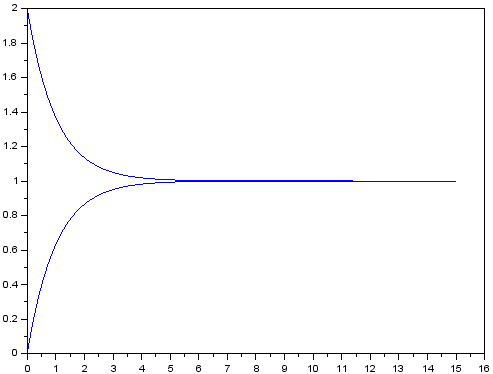
\includegraphics{../../Pictures/control/a5}
	\caption{Los tres comportamiento}
	\label{fig:../../Pictures/control/a5}
\end{figure}\\

\newpage\section{CONCLUSIÓN}
ERNESTO PRADO RODRÍGUES:

En un sistema de primer orden se aprecia su comportamiento y tendencia o estabilidad mediante la constante de tiempo y la ganancia del sistema, los cuales nos indicaran en que tiempo y momento serán estables o si no lo son.
Aplicamos la transformada de laplace para la solución del sistema que nos dio una ecuación en el domino de laplace conocida como función de transferencia. Lo que me ayudo mucho para entender el comportamiento, fue el graficar la función y podrían existir perturbaciones tales como impulso, escalón y rampa.
En este sistema en especial, que fue resuelto y analizado, en lo personal, me ayudo a entender los problemas o que se pueden analizar con otros sistemas distintos que tienen una similitud y que nos arrojan los mismos resultados, en este caso fue de un sistema que básicamente consistía en llenar un tinaco y que pasaba cuando tenia una salida mayor, igual y menor que la entrada, tal sistema hicimos la analogía con circuitos, que de igual manera se analizaron dependiendo del resultado que se quisiera de la entrada y salida ya sea de voltaje o corriente.

JUAN PABLO LEÓN PASCUAL

Un sistema hidráulico se puede modelar con un circuito eléctrico ya que tiene el mismo comportamiento, se analizo el llenado de un tinaco cuando la entrada al sistema era mayo menor e igual.
Esta analogía lo traslada a un sistema de primer orden donde se proporciona una entrada y se obtiene una salida en el dominio de la transformada de laplace y obtener un función de transferencia para el control del mismo sistema. comparamos las grafiacas donde la  entrada al sistema era mayor y proporciona una salida menor esto por la superficie de salida del tinaco. 
el pocas palabras un sistema de primer orden describe el comportamiento y la estabilidad  mediante los factores, de la constante de tiempo y la ganancia del sistema.

\section{BIBLIOGRAFÍA}
Bolton, W., & Ramírez, F. J. R. (2001). Ingeniería de control. Marcombo.

Smith, C. A., Corripio, A. B., & Basurto, S. D. M. (1991). Control automático de procesos: teoría y práctica (No. 968-18-3791-6. 01-A3 LU. AL-PCS. 1.). Limusa.

Nise, N. S., & Romo, J. H. (2002). Sistemas de control para ingeniería (pp. 614-635). Cecsa.

Dale E. Seborg, “Process Dynamics and Control”. Sistemas de 1
er 
Orden. 2ª Edición. Ed. John Wiley & Sons


http://www.cartagena99.com/recursos/alumnos/apuntes/Cap_5_SDx.pdf

https://es.slideshare.net/AnngeeLiiToO/estudio-paramtrico-de-un-sistema-dinmico-de-primer-orden

\end{document}